\documentclass[convert={outfile=\jobname.png}]{standalone}
\usepackage{base}
\usepackage{draw}
\usepackage{code}

\begin{document}

\newcommand{\ga}{
    \begin{tikzpicture}[scale=.4]
        \draw (0, 0) rectangle (1, 1);
    \end{tikzpicture}
}
\newcommand{\gb}{
    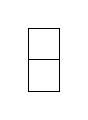
\begin{tikzpicture}[scale=.4]
        \draw (0, 0) rectangle (1, 2);
        \draw (0, 1) to (1, 1);
    \end{tikzpicture}
}
\newcommand{\gc}{
    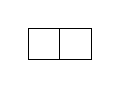
\begin{tikzpicture}[scale=.4]
        \draw (0, 0) rectangle (2, 1);
        \draw (1, 0) to (1, 1);
    \end{tikzpicture}
}
\newcommand{\gd}{
    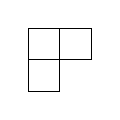
\begin{tikzpicture}[scale=.4]
        \draw (0, 1) rectangle (2, 2);
        \draw (0, 0) rectangle (1, 2);
    \end{tikzpicture}
}
\begin{tikzpicture}[level distance=15mm,
    level 1/.style={sibling distance=3cm},
    level 2/.style={sibling distance=1.5cm}]
\node[circle, draw] (r) { \begin{tikzpicture}[scale=.4]
    \foreach \x in {0, ..., 2} {
        \draw (\x, 0) -- (\x, 2);
        \draw (0, \x) -- (2, \x);
    }
    \end{tikzpicture}
}
child { node[circle, draw] {\ga} }
child { node {\gb} 
    child {node {\ga}}
}
child { node {\gc} 
    child {node {\ga}}
}
child { node[circle, draw] {\gd} 
    child {node[circle, draw] {\gb}
        child {node[circle, draw] {\ga} }
    }
    child {node[circle, draw] {\gc}
        child {node[circle, draw] {\ga} }
    }
};
\node at (-6, 0) {Alice};
\node at (-6, -1.5) {Bob};
\node at (-6, -3) {Alice};
\node at (-6, -4.5) {Bob};
\end{tikzpicture}
\end{document}
